% !TeX root = ../../../book.tex

\subsection{乘法原理}

\subsubsection*{引言}

我们通过一个具体例子引入乘法原理。

\begin{example}
    假设房间里有三个人和三张贴纸,每张贴纸上分别标有数字 $1, 2, 3$。那么,有多少种不同的方式可以将这些贴纸分配给这三个人?为了便于讨论,不妨将三人分别称为 Andy、Brendan 和 Carl,简记为 $A, B, C$。我们可以系统地列出所有可能的贴纸分配方式,以确保不重复、不遗漏。具体来说,让 Andy 先选,接着是 Brendan,最后是 Carl,得到 $(A, B, C) = $
    \[(1, 2, 3) \quad (1, 3, 2) \quad (2, 1, 3) \quad (2, 3, 1) \quad (3, 1, 2) \quad (3, 2, 1)\]
    % \begin{itemize}
    %     \item $(1, 2, 3)$
    %     \item $(1, 3, 2)$
    %     \item $(2, 1, 3)$
    %     \item $(2, 3, 1)$
    %     \item $(3, 1, 2)$
    %     \item $(3, 2, 1)$
    % \end{itemize}
    因此,总共有 $6$ 种不同的分配方式。

    如果现在有四个人和四张贴纸呢?我们是否还能列出所有分配方式?当然可以。
    \begin{align*}
        (1, 2, 3, 4) \quad (1, 2, 4, 3) \quad (1, 3, 2, 4) \quad (1, 3, 4, 2) \quad (1, 4, 2, 3) \quad (1, 4, 3, 2) \\
        (2, 1, 3, 4) \quad (2, 1, 4, 3) \quad (2, 3, 1, 4) \quad (2, 3, 4, 1) \quad (2, 4, 1, 3) \quad (2, 4, 3, 1) \\
        (3, 1, 2, 4) \quad (3, 1, 4, 2) \quad (3, 2, 1, 4) \quad (3, 2, 4, 1) \quad (3, 4, 1, 2) \quad (3, 4, 2, 1) \\
        (4, 1, 2, 3) \quad (4, 1, 3, 2) \quad (4, 2, 1, 3) \quad (4, 2, 3, 1) \quad (4, 3, 1, 2) \quad (4, 3, 2, 1)
    \end{align*}
    所以总共有 $24$ 种不同的分配方式。那如果是五个人呢?不管你怎么想,反正我光是列出这些方案就已经手酸了。一定存在更好的方法!没错,这时就该乘法原理登场了。
\end{example}
(旁注:你可能已经注意到上面的列表存在某种规律;你能看出我们是如何确保不遗漏任何情况的吗?你能尝试编写一个程序,对任意给定人数生成所有可能的分配方式吗?动手试试吧!)

\subsubsection*{陈述}

实际上,我们将从两个角度阐述乘法原理:第一个是直观且易于应用的版本,第二个是基于集合论的严格数学表述。需要强调的是,理想情况下两者都应掌握,但理解直观版本更为重要,因为严格版本主要用于数学证明。

\begin{proposition}
    考虑一个由 $n$ 个独立步骤组成的过程。假设对于每一个 $i \in [n]$,第 $i$ 步恰好有 $w_i \in \mathbb{N}$ 种不同的完成方式,并且该数目不依赖于前面各步所做出的选择。假设在任意一步中,不同的选择都会导致不同的最终结果。那么,乘法原理指出,整个过程的总结果数 $N$ 为
    \[N = \prod_{i \in [n]} w_i\]
\end{proposition}

在进一步严格表述乘法原理之前,让我们先回顾之前分配贴纸的例子。

\begin{example}
    将贴纸分配给 Andy、Brendan 和 Carl 的过程可以视为一个三步操作:首先按字母顺序(从左到右)对三人排序,然后依次分配贴纸。每一步中,我们从未分配的贴纸中选一张分配给当前的人。

    第一步,我们来到 Andy 面前,有 $3$ 张贴纸可选。

    第二步,我们来到 Brendan 面前,无论之前选了什么,此时都剩下 $2$ 张贴纸可选。注意,无论 Andy 拿到的是 $1$、$2$ 还是 $3$,Brendan 的可选数量始终为 $2$。

    第三步,我们来到 Carl 面前,无论此前两步如何选择,都只剩 $1$ 张贴纸可选。

    根据乘法原理,完成整个分配过程的方法数为各步选择数的乘积:$3 \times 2 \times 1 = 6$。这与我们之前``穷举所有可能''得到的结果一致。太棒了!

    如果是 $4$ 个人呢?运用相同的逻辑,分配方式数为 $4 \times 3 \times 2 \times 1 = 24$,也与之前列出的结果一致。完美!

    如果是 $5$ 个人呢?那么结果为 $5 \times 4 \times 3 \times 2 \times 1 = 120$。我们得到了一个新的结论,着实令人惊喜!如果是 $6$ 个人呢?$7$ 个人呢?甚至任意 $n \in \mathbb{N}$ 个人呢?幸亏有乘法原理,我们现在可以轻松而准确地回答这些问题。这真是太棒了!
\end{example}
\subsubsection*{树状图}

\emph{树状图}能够以生动直观的方式阐释乘法原理。树的概念源于数学中的\emph{图论},这门学科研究由顶点(点)和边(连接点的线段)构成的数学对象,其中只关注边是否存在,而不考虑其具体形态。树是一类特殊的图,在计算机科学中极为常见,尤其在研究\emph{分支过程}时广泛应用。在讨论乘法原理时,我们可以借助树来表示决策过程中的各个节点,并利用乘法原理计算可能的结果数目。此外,这种方法还有助于我们理解乘法原理的严谨数学表述与证明。(我们将这些更深层次的目标留作练习,但对于有兴趣的读者,我们强烈推荐阅读本节内容,它将为你提供直观的理解并指导你完成相关练习。)

\begin{example}
    让我们通过一个具体例子探讨树状图与乘法原理之间的关系。假设我们需要为下学期安排选课。根据专业要求、时间限制和个人兴趣,我们必须从数学、计算机科学和哲学三个系中各选一门课程。每个系的课程数量相互独立:具体而言,有 $4$ 门数学课程、$3$ 门计算机课程和 $2$ 门哲学课程可供选择,且只要满足每个系各选一门课,任何课程组合都不会出现时间冲突。

    如何应用乘法原理呢?首先需要定义一个完整的\emph{过程}及其若干\emph{步骤},并确定每一步的选择数目。总体过程是确定下学期的课程安排。由于必须从每个系中选择一门课程,我们可以将过程划分为三个步骤:
    \begin{enumerate}
        \item 选择一门数学课程;
        \item 选择一门计算机课程;
        \item 选择一门哲学课程。
    \end{enumerate}(注意:这些步骤的顺序是否重要?如果先选择哲学课程,过程会有本质区别吗?我们认为不会,但在继续阅读之前,请确保你理解其中的原因。)

    接下来明确每一步的选择数目。设 $4$ 门数学课程集合为 $\mathcal{M} = \{M_1, M_2, M_3, M_4\}$,$3$ 门计算机课程集合为 $\mathcal{C} = \{C_1, C_2, C_3\}$,$2$ 门哲学课程集合为 $\mathcal{P} = \{P_1, P_2\}$。于是:
    \begin{enumerate}
        \item \quad 数学课程有 $4$ 种选择;
        \item 计算机课程有 $3$ 种选择;
        \item \quad 哲学课程有 $2$ 种选择。
    \end{enumerate}
    根据乘法原理,总的课程安排方式为 $4 \times 3 \times 2 = 24$ 种。那么,为什么会有如此多的可能性?这些具体安排是怎样的?让我们通过树状图来可视化这一过程!

    \begin{center}
        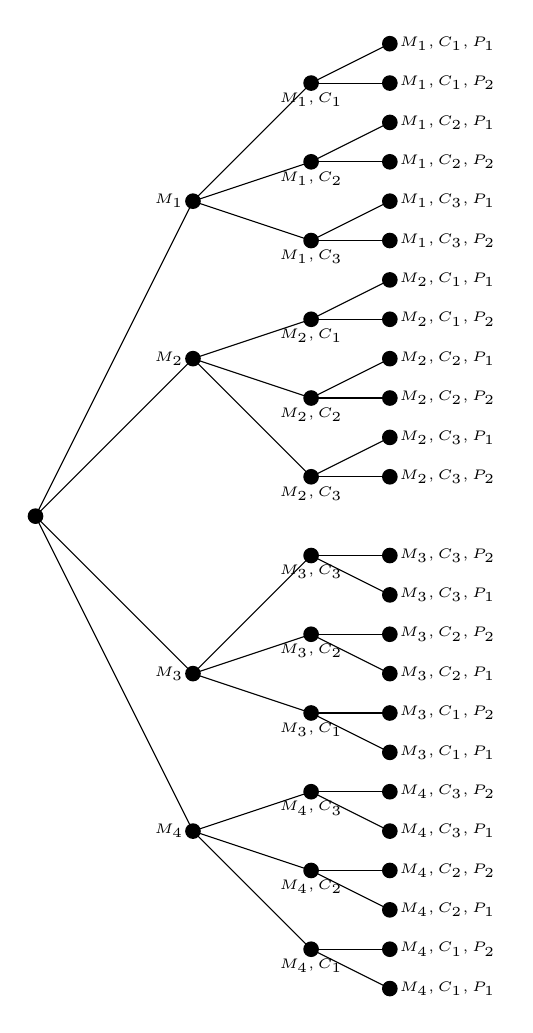
\begin{tikzpicture}[scale=0.5]
            \node at (0, 0)[circle,fill,inner sep=2pt]{};
            \foreach \m in {1,2,-1,-2}
            {
            \pgfmathparse{(\m>0) ? 1 : -1};
            \edef\direction{\pgfmathresult};
            \edef\my{\m*4};
            \node at (4, \my)[circle,fill,inner sep=2pt]{};
            \pgfmathparse{(\m>0) ? int(3-\m) : int(2-\m)};
            \edef\i{\pgfmathresult};
            \node[left] at (4, \my){\tiny $M_{\i}$};
            \foreach \c in {0,1,2}
            {
            \edef\cy{\m*6-5*\direction+\c*2*\direction};
            \node at (7, \cy)[circle,fill,inner sep=2pt]{};
            \pgfmathparse{int(3-\c)};
            \edef\j{\pgfmathresult};
            \node[below] at (7, \cy){\tiny $M_{\i},C_{\j}$};
            \foreach \p in {0,1}
            {
            \edef\dy{\cy+\p*\direction};
            \node at (9, \dy)[circle,fill,inner sep=2pt]{};
            \pgfmathparse{int(2-\p)};
            \edef\k{\pgfmathresult};
            \node[right] at (9, \dy){\tiny $M_{\i},C_{\j},P_{\k}$};
            \draw (9, \dy) -- (7, \cy);
            }
            \draw (7, \cy) -- (4, \my);
            }
            \draw (4, \my) -- (0, 0);
            }
        \end{tikzpicture}
    \end{center}

    从左到右阅读树状图,即对应我们定义的三步过程。最左侧的单个顶点表示起点——此时尚未做出任何选择。从该顶点延伸出的四条边分别对应四门数学课程,每条边标记为 $\mathcal{M}$ 中的一个元素。无论选择哪条边(即哪门数学课程),下一个顶点都会延伸出三条边,对应三门计算机课程,边上标记着 $\mathcal{C}$ 的相应元素。类似地,每个后续顶点再延伸出两条边,标记为 $\mathcal{P}$ 的相应元素。

    树状图的优势在于能够清晰展示全部 $24$ 种结果。例如,最右上方的顶点对应选择 $M_1$、$C_1$ 和 $P_1$,可用有序三元组 $(M_1, C_1, P_1)$ 表示;其下方的顶点则对应 $(M_2, C_3, P_1)$。每个末端顶点都唯一对应一个有序三元组!应用乘法原理时,我们实际上是在计算若干集合的\emph{笛卡尔积}的基数。该过程即识别集合中的元素并将它们组合成有序元组。乘法原理表明,通过计算所有此类元组构成集合的基数,即可得到所有可能排列的总数。在本例中,我们有:
    \[|\mathcal{M} \times \mathcal{C} \times \mathcal{P}| = |M| \cdot |C| \cdot |P| = 4 \cdot 3 \cdot 2 = 24\]

    现在你是否觉得这种解释更加清晰?它能否帮助你更好地理解乘法原理的实际应用?
\end{example}

\subsubsection*{更正式的陈述}

请参见练习 \ref{exc:exercises8.9.1},该练习要求证明以下定理。这是乘法原理在数学上更正式的表述。在陈述定理之后,我们将解释其与先前版本的联系。

\begin{theorem}[乘法原理(集合论版本)]\label{theorem8.2.10}
    设 $n \in \mathbb{N}$。假设 $\forall i \in \mathbb{N} \centerdot T_i$ 为有限集。则
    \[\left|\prod_{i \in [n]} T_i \right| = |T_1 \times T_2 \times \dots \times T_n| = |T_1| \cdot |T_2| \cdot \dots \cdot |T_n| = \prod_{i \in [n]} |T_i|\]
\end{theorem}

该定理与先前所述的乘法原理之间的联系如下:集合 $T_1$ 的元素代表步骤 $1$ 中可做出的选择;对于 $T_1$ 的每一元素,我们定义集合 $T_2$ 表示在步骤 $1$ 做出选择\emph{之后},步骤 $2$ 中可做出的选择。假设无论步骤 $1$ 的选择如何,步骤 $2$ 中的选择数量均相同,因此定理结论只涉及 $|T_i|$ 是合理的,因为这个值是明确的。同理,$T_3$ 表示在步骤 $1$ 和 $2$ 之后步骤 $3$ 中可做出的选择,且假设 $|T_3|$ 也是明确的。

最终,我们可以用一个有序 $n$ 元组来描述该过程的\textbf{输出},其中第 $i$ 个坐标为集合 $T_i$ 的一个元素。尽管该元素依赖于先前的坐标,但其选择\textbf{数量}与之前的选择无关。由于我们最终只关心可能结果的\textbf{数量},因此该结论是合理的。实际上,\textbf{列出}所有结果需要仔细分析每一步,观察特定选择如何影响后续步骤的选择,但这不是结论的重点。正因如此,实质上该结果证明了有限集笛卡尔积的大小等于它们大小的乘积。

\subsubsection*{示例:应用加法和乘法原理}

让我们练习使用这两条原理。为了方便引用,我们将这两条原理分别缩写为 ROS (加法原理)和 ROP (乘法原理)。请注意,每次使用时我们均会明确引用它们!

\begin{example}[车牌]
    假设车牌字符串由 $6$ 或 $7$ 个字符组成,每个字符为字母($A$ 至 $Z$)或数字($0$ 至 $9$)。
    \begin{enumerate}[label=(\arabic*)]
        \item 总共可以有多少张车牌?

              我们需要根据字符串的长度,分为 $6$ 位和 $7$ 位两种情况。

              对于每种情况,我们有一个包含 $6$ 步或 $7$ 步的过程。在第 $i$ 步,我们从 $36$ 个选项($26$ 个字母和 $10$ 个数字)中选择一个字符填入第 $i$ 位。

              因此,根据 ROP,长度为 $6$ 的字符串有 $36^6$ 种可能,长度为 $7$ 的字符串有 $36^7$ 种可能。

              再根据 ROS,车牌字符串总数为 $36^6 + 36^7$。\\
        \item 有多少车牌最多包含一个数字?

              我们需要根据包含 $0$ 个数字或 $1$ 个数字划分成两种情况。
              \begin{itemize}
                  \item 如果没有数字,在每一步中我们都会在相应位置填入一个字母。根据 ROP,长度为 $6$ 的字符串有 $26^6$ 种可能,长度为 $7$ 的字符串有 $26^7$ 种可能。

                        根据 ROS,总共有 $26^6 + 26^7$ 种可能。
                  \item 如果包含 $1$ 个数字,首先在步骤 $1a$ 中选择哪个位置用数字填充,然后在步骤 $1b$ 中选择具体的数字,其余位置都用字母填充。

                        这种情况下,对长度为 $6$ 的字符串,有 $6$ 种选择数字位置的方式、$10$ 种选择数字的方式,其余 $5$ 个位置各有 $26$ 种选择;对长度为 $7$ 的字符串,有 $7$ 种选择数字位置的方式、$10$ 种选择数字的方式,其余 $6$ 个位置各有 $26$ 种选择。
                        
                        根据 ROS 和 ROP,总共有 $(6 \cdot 10 \cdot 26^5) + (7 \cdot 10 \cdot 26^6)$ 种可能。
              \end{itemize}
              综上,根据 ROS,总共有
              \[(26^6 + 6 \cdot 10 \cdot 26^5) + (26^7 + 7 \cdot 10 \cdot 26^6)\]
              种可能的结果。\\
        \item 有多少车牌至少包含两个数字?

              我们可以仿照上面的方法,将此类车牌按数字个数($3$ 至 $7$ 个)划分,再计算每个集合的大小并求和。例如,对包含 $4$ 个数字的车牌,需要从 $6$ 个位置中选择 $4$ 个位置放置数字——此时二项式系数将派上用场(在我们定义并推导出公式之后)。

              我们可以复用刚才的工作成果!将所有车牌(集合 $Y$)划分为最多包含 $1$ 个数字的车牌(集合 $X_1$)与至少包含 $2$ 个数字的车牌(集合 $X_2$)。由于这是一种划分,由 ROS 可得 $|Y| = |X_1| + |X_2|$。通过代数运算,我们得到如下表达式:
              \begin{align*}
                  |X_2| & = |Y| - |X_1|                                                                       \\
                        & = (36^6 + 36^7) - [(26^6 + 6 \cdot 10 \cdot 26^5) + (26^7 + 7 \cdot 10 \cdot 26^6)]
              \end{align*}
              只需代入已经推导出的表达式即可。这种方法极为便捷!

              通常来说,这是一种有效的策略:为了计算某个集合的大小,可以先计算其补集(即该集合外所有``其他''元素构成的集合),再从``总数''中减去补集元素的数量。然而,需要注意的是,我们目前只能使用加法原理,尚未引入减法原理,所以我们需要始终通过\emph{划分}与\emph{加法}表达此过程。待减法原理引入后,我们便可以直接对数值或代数变量进行减法运算;最终,随着数学能力的提升,我们可以跳过这些形式化步骤,直接谈论``减去''某一数量。但目前为了强调计数方法的基础,我们需要谨慎地运用加法原理并采用准确的措辞。\\
        \item 有多少车牌不包含元音字母及偶数数字?

              这种情况限只是制了每一步的选择数量:每个位置仅可从 $21$ 个非元音字母与 $5$ 个奇数数字中选择,共 $26$ 种选项。所以根据 ROP 与 ROS,总共有
              \[26^6 + 26^7\]
              种可能的结果。
    \end{enumerate}
\end{example}